%!TEX root = ../Thesis.tex

\section{Spur-Geometrie Bestimmung}
\label{cha:lane_definition}

Nachfolgend wird beschrieben, wie aus den identifizierten Trajektorie-Clustern
Geometrie-Informationen der Fahrspuren abgeleitet werden. Eine Spur-Geometrie besteht grundsätzlich
aus einer Mittellinie und zwei Hülllinien, welche die Breite der Spur festlegen.
Bestimmt werden die Geometrien primär in drei Schritten:

\begin{itemize}
    \item Bestimmung der Spur-Mittellinien,
    \item Bestimmung der Spurhüllen und
    \item Partitionierung sich überlagernder Spuren.
\end{itemize}

Hinzu kommen weitere Zwischenschritte. Die wichtigsten werden ebenfalls nachfolgend beschrieben.

\subsection{Ausfilterung von Spurwechselvorgängen}
\label{sec:real2_filter_lane_change}

Bevor mithilfe der im vorherigen Schritt gewonnenen Trajektorie-Cluster Mittellinien von Fahrspuren bestimmt
werden können, müssen diese nochmals vorverarbeitet werden. Die einzelnen Cluster enthalten teilweise
Bewegungsbahnen, welche Spurwechselvorgänge oder andere Abweichungen von einer Fahrspur beschreiben.
Diese Trajektorien müssen, so weit wie möglich,
entfernt werden, da sie die anschließende Geometrie-Bestimmung negativ beeinflussen. Die Trajektorien
eines Clusters sollten möglichst eindeutig einer realen Fahrspur zuzuordnen sein. In Abbildung
\ref{fig:real2_clusters_pre_postpro} sind beispielhaft zwei Cluster dargestellt, welche eine Vielzahl an
Spurwechselvorgängen enthalten.

\begin{figure}[H]
    \centering
    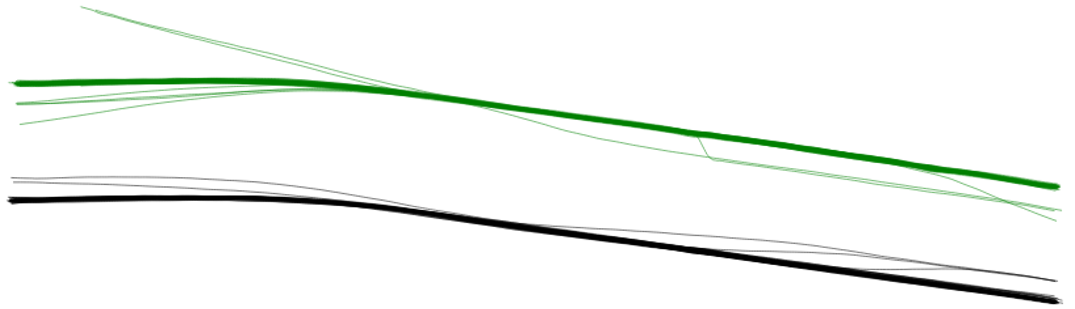
\includegraphics[width=0.8\linewidth]{resources/img/umsetzung/U2/Clusters_Pre_Postprocessing}
    \caption{Trajektorie-Cluster mit Spurwechselvorgängen}
    \label{fig:real2_clusters_pre_postpro}
\end{figure}

Die Grundidee, welche der Ausfilterung der Abweichungen zugrunde liegt, ist, jene Trajektorien
aus einem Cluster zu entfernen, welche eine überdurchschnittlich hohe mittlere Distanz zu allen anderen
Trajektorien des Clusters besitzen. Als Distanzmaß wird erneut die LCSS-Distanz verwendet.
Ein ähnlicher, Distanz-basierter Ausreißer-Detektionsansatz wird in \cite[]{Mirge2017} vorgestellt.
Der in dieser Arbeit verwendete Algorithmus ist in Listing \ref{lst:pseudo_post_processing} beschrieben.

\begin{lstlisting}[caption=Pseudocode Cluster Post-Processing, language=Pseudo, label=lst:pseudo_post_processing]
algorithm filterCluster:
  input:  unfiltered trajectories of cluster: trajsIn
  output: filtered trajectories of cluster

  meanTrajectoryDistances :=
    for each traj in trajsIn do
      yield mean LCSS distance of traj to all other trajectories of trajsIn
    end

  clusterCmpVal := select median of meanTrajectoryDistances as comparison value

  resultTrajs :=
    for each traj in trajsIn do
      if meanDist of traj < 1.5 * clusterCmpVal then
        yield trajs
      end
    end

  return resultTrajs
\end{lstlisting}

Das gewählte Verfahren ist einfach, eignet sich aber gut, um das gewünschte Ziel zu erreichen.
Die in Abbildung \ref{fig:real2_clusters_post_postpro} dargestellten Ergebnisse zeigen dies.
Aus den in Abbildung \ref{fig:real2_clusters_pre_postpro} enthaltenen Clustern wurden alle Trajektorien
mit Spurwechselvorgängen oder Abweichungen entfernt. Die Effektivität konnte auch durch die Anwendung
auf andere Datensätze bestätigt werden.
Wenn in einem Cluster viele Trajektorien Abweichungen von einer Spur besitzen, ist es möglich, dass der Algorithmus
diese nicht vollständig entfernt. Bei einer geringen Anzahl von Abweichungen oder Ausreißer arbeitet
er allerdings zuverlässig.

\begin{figure}[H]
    \centering
    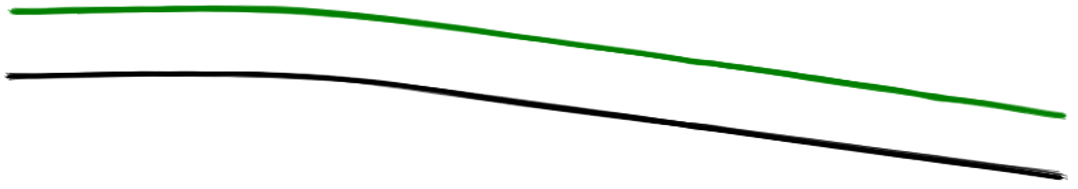
\includegraphics[width=0.8\linewidth]{resources/img/umsetzung/U2/Clusters_Post_Postprocessing}
    \caption{Bereinigte Trajektorie-Cluster ohne Spurwechselvorgänge}
    \label{fig:real2_clusters_post_postpro}
\end{figure}

Zu beachten ist, dass die Zeitkomplexität des Verfahrens bei großen Trajektorie-Clustern
nicht unerheblich ist. Dies ist auf die Komplexität des LCSS Distanzmaßes zurückzuführen.
Bei der Untersuchung alternativer Vorgehensweise wurde allerdings klar, dass es grundlegend schwer ist,
das Problem der Ausreißer-Erkennung performant zu lösen.
In \cite[]{Meng2018} werden hierzu diverse Distanz- und Dichte-basierte
Arbeiten vorgestellt und verglichen. Da diese alle allerdings nicht weniger komplex sind und häufig
die verfolgten Ziele über die hier geforderten hinausgehen, wurde entschieden den oben beschriebenen Ansatz
zu verwenden. Durch die Parallelisierung der Berechnung der mittleren Abstände konnte die Performance
des Ansatzes außerdem nochmals deutlich gesteigert werden.

\subsection{Bestimmung der Spurmittellinien}
\label{sec:real2_define_lane_centerline}

Nachdem die Trajektorie-Cluster nun weitestgehend von Fahrspurwechseln und anderen Abweichungen bereinigt
wurden, beschreiben die verbleibenden Bewegungsbahnen eines Clusters eine Fahrspur.
Anhand dieser Trajektorien können daher nun die Mittellinie der Spuren bestimmt werden.

Die gesuchten Mittellinien verlaufen durch die Mitte der entsprechenden
Trajektorie-Cluster. Die einzelnen Bewegungsbahnen besitzen jeweils leichte Abweichungen von dieser \textit{``Ideallinie''}.
Als Spurmittellinie -- wie von \cite{Hu2005} vorgeschlagen -- jene Trajektorie zu wählen, welche die
kleinste Summe der Distanzen zu allen anderen Trajektorien eines Clusters besitzt, ist nicht praktikabel,
da die so gefunden Trajektorie nicht über ihre komplette Länge in der Mitte des Clusters verlaufen muss
und auch nicht zwangsläufig so lang ist, wie die anderen Trajektorien des Clusters.
Auf eine Bestimmung der Mittellinie mittels linearer oder polynomialer Regression, wie beispielsweise in
\cite[]{Chen2014} oder \cite[]{Melo2006} angewandt,
wurde ebenfalls verzichtet. Der Grund hierfür ist, dass einerseits die Komplexität und Form der Fahrbahnverläufe
nicht bekannt ist und andererseits das Erlernen der Spurrepräsentationen auf diese Weise sehr aufwendig ist.

Der in dieser Arbeit gewählte Ansatz zur Bestimmung der Mittellinien macht sich die von Atev et al.
vorgestellte Notation einer relativen Position innerhalb einer Trajektorie zu nutze, welche in
Gleichung \ref{eq_atev_relPos} und \ref{eq_atev_findPointAtRelPow} gegeben ist.
Die Koordinaten der Spurlinien ergeben sich aus den Mittelwerten von Trajektorie-Punkten, welche sich
alle an der selben relativen Position befinden. Vorteil der Verwendung der relativen Positionen ist,
dass Punkte auf Trajektorien mit einer Position $p_r$ auch dann auf der selben Höhe liegen,
wenn die Bahnen aufgrund von Oszillationen um die Spurmitte unterschiedliche Längen haben.
Der verwendete Algorithmus ist nachfolgend beschrieben.
\begin{lstlisting}[caption=Pseudocode Mittellinien-Bestimmung, language=Pseudo, label=lst:pseudo_centerline_definition]
algorithm calculateCenterline:
  input:  trajectories of cluster: trajsIn
  output: centerline of lane

  meanTrajLength := calculate mean point length of trajectories
  relPositions := define range with relative positions of size meanTrajLength
                  and step-size (1 / meanTrajLength)

  centerline :=
    for each relP in relPositions do
      pointsAtRelPos := get points at relP (*for each*) traj (*in*) trajsIn
      yield mean of all points (*in*) pointsAtRelPos
    end

  return centerline
\end{lstlisting}

Da die Form und der Verlauf von Trajektorien eines Clusters sich nur wenig unterscheiden, liefert dieses
Vorgehen gute Ergebnisse. In Abbildung \ref{fig:real2_results_centerline_detection} a) ist beispielhaft
dargestellt, wie eine Mittellinien innerhalb eines Trajektorie-Clusters verläuft.
In \ref{fig:real2_results_centerline_detection} b) sind alle Spurmittellinien in der Neckartor-Kreuzung abgebildet,
welche auf die oben beschriebene Weise bestimmt wurden.

\begin{figure}[H]
    \centering
    \subfloat[]{{
        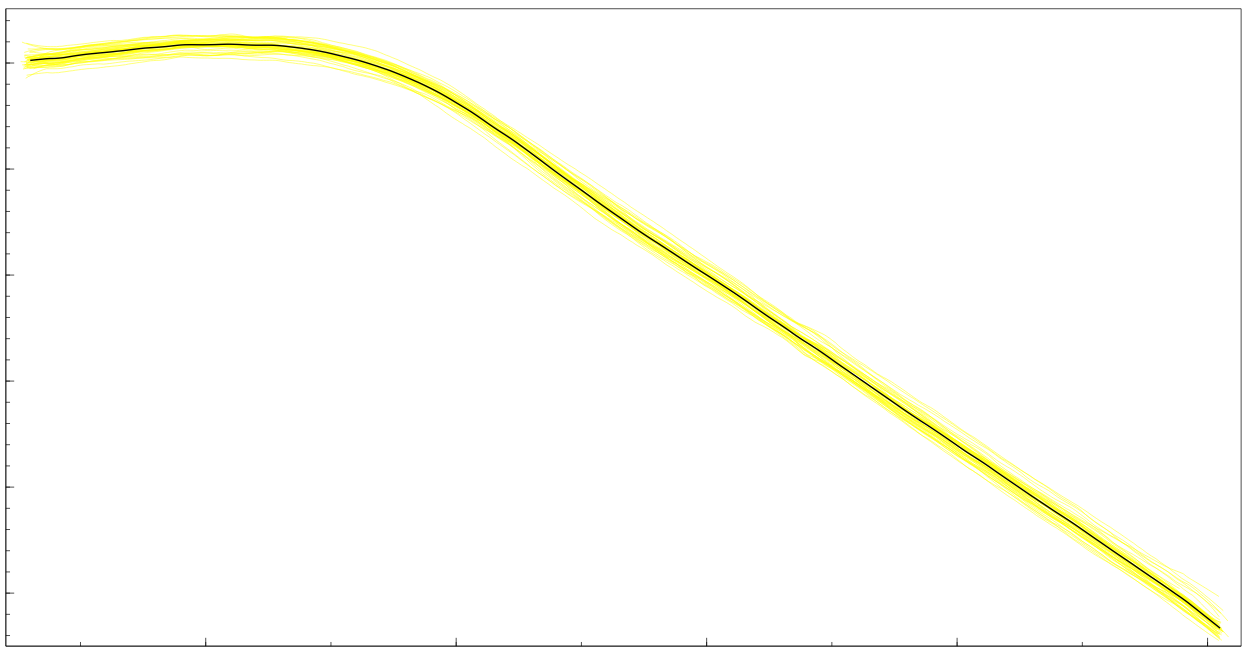
\includegraphics[align=c, width=0.35\linewidth]{resources/img/umsetzung/U2/cluster_with_centerline}
    }}
    \qquad
    \subfloat[]{{
        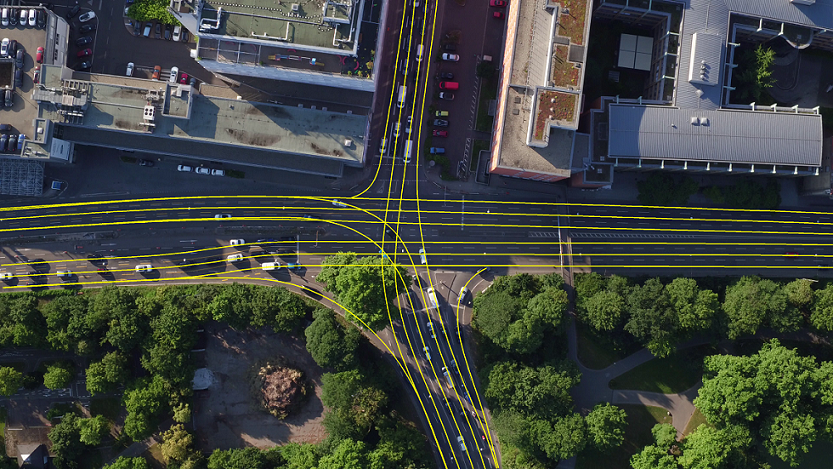
\includegraphics[align=c, width=0.5\linewidth]{resources/img/umsetzung/U2/laneCentersInImage}
    }}
    \caption[Ergebnisse Spurmittellinien-Bestimmung]{Spurmittellinie in einem Trajektorie-Cluster a), Spurmittellinien Neckartor-Kreuzung b)}
    \label{fig:real2_results_centerline_detection}
\end{figure}

Das beschriebene Verfahren kann, im Gegensatz zu den meisten Ansätzen welche in den verwandten Arbeiten zum Einsatz kommen,
Spurmittellinien für unterschiedlichste Spurverläufe ermitteln. 
Diese werden, da es sich bei ihnen ebenfalls um Sequenzen von 2D-Koordinaten handelt,
im Algorithmus über Trajektorie-Objekte repräsentiert (siehe Abbildung \ref{fig:real_trajectory_classDia}).

\subsection{Angleichung benachbarter Spurenden}

Bevor für jede Spurmittellinie eine Hülle definiert wird,
werden benachbarte Spurenden aneinander angeglichen. Diese sollen immer auf der selben Höhe beginnen
beziehungsweise enden, um die Positionen von Fahrzeugen auf benachbarten Spuren bei der
Verkehrsanalyse besser vergleichen zu können.

Benachbarte Fahrspuren können einen deutlich sichtbaren Versatz an ihren Anfängen
und Enden besitzen, was beispielsweise in Abbildung \ref{fig:real2_lane_alignment} a) dargestellt ist.
Diese Unterschiede entstehen
primär, da Fahrzeuge am Rand der Aufnahme verschieden schnell erkannt werden und so deren Trajektorien
unterschiedlich früh beginnen. Für das Angleichen der Spurenden sind grundlegend drei Schritte notwendig:
Finden von benachbarten Enden, Bestimmung der längsten Spur im Bereich der Enden und schließlich das
Angleichen aller Spuren auf die Höhe der vorher bestimmten ``äußersten'' Mittellinie.

Gruppen benachbarter Spurenden werden auf rekursive Weise gefunden. Es wird eine Spur gewählt und im
Bereich ihres Starts beziehungsweise Endes nach unmittelbaren Nachbarn gesucht. Das hierzu verwendete
Verfahren ist in Abschnitt \ref{sec:real2_identify_parallel_lanes} beschrieben. Für jede der so gefundenen
Nachbarspuren wird wiederum nach deren Nachbarn gesucht. Auf diese Weise ergibt sich eine Spur-Gruppe.

Da das Weltkoordinatensystem in den verwendeten Aufnahmen keine feste Orientierung und keinen fixen Ursprung besitzt,
kann die in einer Spur-Gruppe am weitesten außen liegende Spur nicht identifiziert werden, indem die
Koordinaten der Start- oder Endpunkte der Spuren verglichen werden.
Bestimmt wird die ``äußerste'' Mittellinie daher, indem durch jeden Endpunkt der Spuren einer Gruppe
eine orthogonale Gerade gelegt wird. Die Spur deren zugehörige Gerade die wenigsten Schnittpunkte
mit anderen Spur-Mittellinien besitzt, liegt am weitesten außen. Abbildung \ref{fig:real2_lane_alignment_concept}
veranschaulicht das Vorgehen.

\begin{figure}[H]
    \centering
    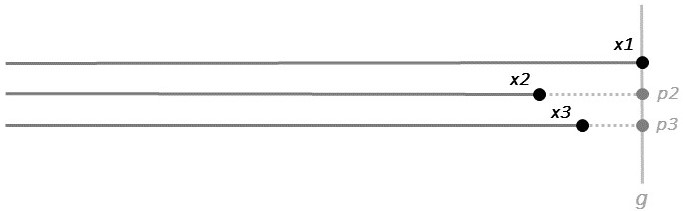
\includegraphics[width=0.5\linewidth]{resources/img/umsetzung/U2/LaneAlignment_concept}
    \caption{Konzept Spurenden-Angleichung}
    \label{fig:real2_lane_alignment_concept}
\end{figure}

Die so bestimmte Gerade $g$ ist zudem gleichzeitig, die Linie, auf welche die anderen Spur-Endpunkte
projiziert werden. Hierzu wird eine Orthogonalprojektion der Endpunkte auf die Gerade $g$ durchgeführt, welche
in Gleichung \ref{eq_orthPro} definiert ist. $\vec r_0$ entspricht hierbei einem Stützvektor auf der Geraden $g$ und
$\vec u$ dem Richtungsvektor.

\begin{ceqn}
\begin{align}
\label{eq_orthPro}
    P_g(\vec x) =  \vec r_0 + \frac{( \vec x - \vec r_0 ) \cdot \vec u}{\vec u \cdot \vec u} \, \vec u
\end{align}
\end{ceqn}

Das Ergebnis der Spurenden-Angleichung ist in Abbildung \ref{fig:real2_lane_alignment} b) dargestellt.

\begin{figure}[H]
    \centering
    \subfloat[]{{
        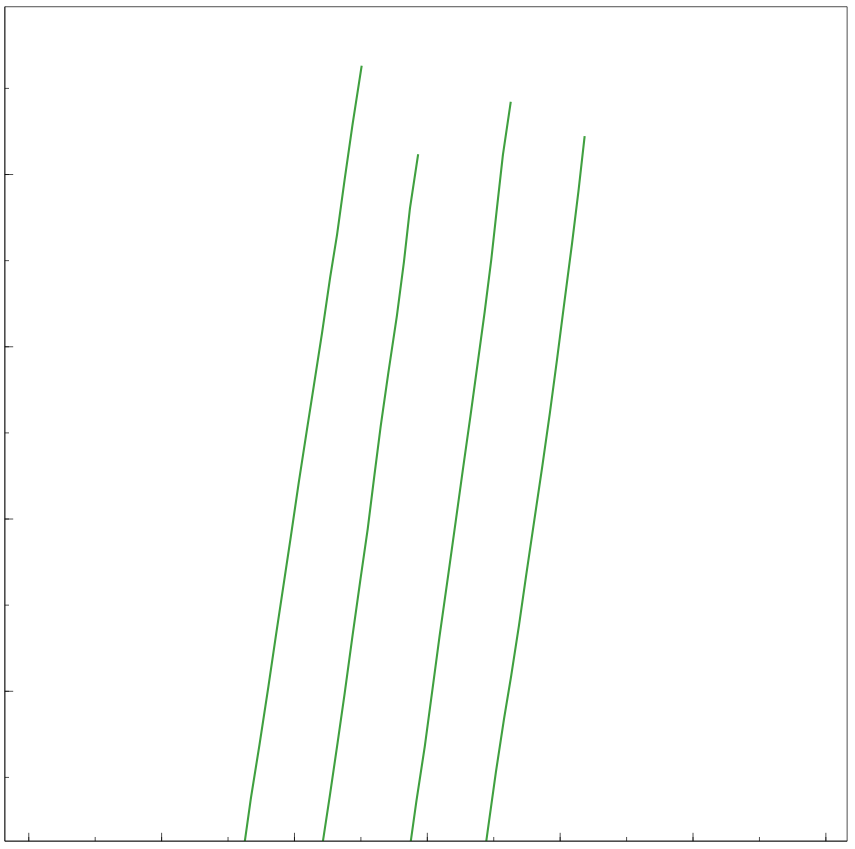
\includegraphics[align=c, width=0.25\linewidth]{resources/img/umsetzung/U2/normalCenterLines}
    }}
    \qquad \qquad
    \subfloat[]{{
        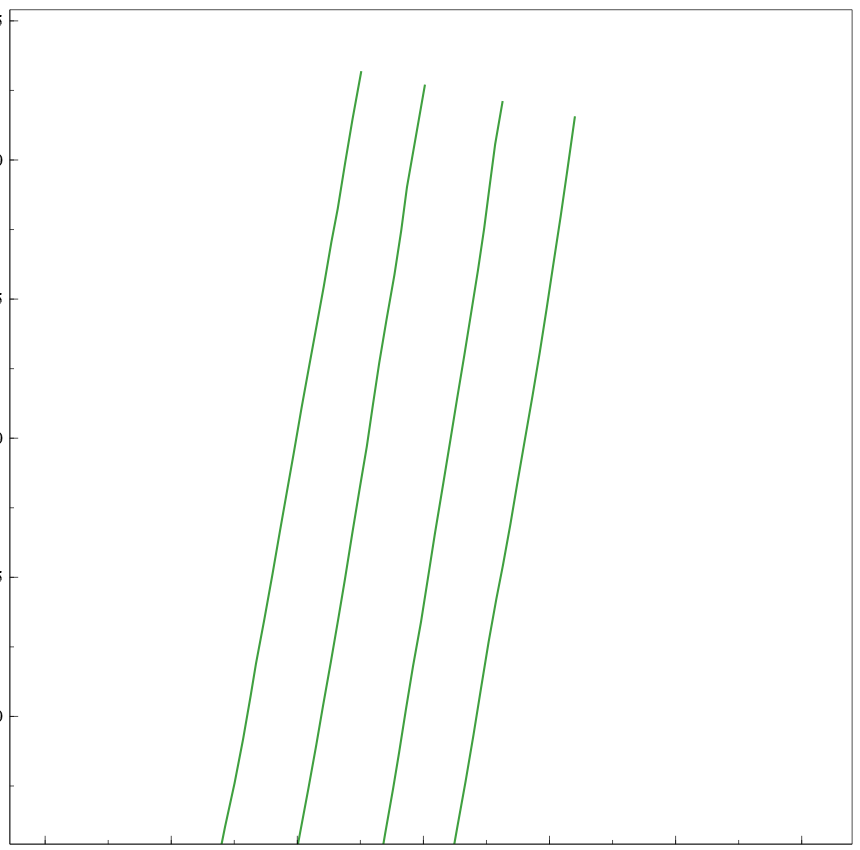
\includegraphics[align=c, width=0.25\linewidth]{resources/img/umsetzung/U2/alignedCenterLines}
    }}
    \caption[Ergebnis Spurenden-Angleichung]{Fahrspur-Mittellinien ohne Angleichung a) und Ergebnis mit Angleichung b)}
    \label{fig:real2_lane_alignment}
\end{figure}

Nachdem die Enden der Spurmittellinien aneinander angeglichen wurden, werden anschließend die Spurhüllen
definiert.

\subsection{Bestimmung der Spurhüllen}
\label{sec:real2_define_lane_envelope}

Auf Basis der vorher bestimmten Mittellinien werden anschließend die Spurhüllen bestimmt.
In folgendem Abschnitt wird das hierzu eingesetzte Verfahren beschrieben.

Eine Spurhülle definiert die Breite einer Fahrbahn. In dieser Arbeit verlaufen sie idealerweise entlang
realer Begrenzungslinien, welche zwei Spuren voneinander oder eine Fahrbahn von einem Seitenstreifen et cetera trennen.
Eine Mittellinie und eine Hülle beschreiben zusammen die Geometrie einer Fahrspur. Diese Geometrie
soll die realen Dimensionen einer Spur möglichst genau abbilden. Aus diesem Grund ist es nicht möglich,
die Hüllen lediglich auf Basis von statistischen Informationen der Trajektorie-Cluster zu bestimmen,
wie das beispielsweise in \cite[]{WeimingHu2006} oder \cite[]{Morris2011} gemacht wird.
Der in dieser Arbeit verwendete Ansatz zur Bestimmung der Spurhüllen basiert daher lediglich auf den
Spurmittellinien und nutzt ihre relative Lage zueinander. Ansätze hierzu stammen aus den Arbeiten von
\cite[]{Hsieh2006} und \cite[]{Makris2005}, welche in Abschnitt \ref{sec:rw_lane_detection} vorgestellt wurden.

Die grundlegende Idee, auf welcher die Bestimmung der Spurhüllen basiert, ist konzeptionell in Abbildung
\ref{fig:real2_envelope_definition_concept} dargestellt.
Für zwei parallel zueinander verlaufende Spuren $l_1$ und $l_2$ werden die Hüllen über den Abstand zwischen
ihren Mittellinien bestimmt. Besitzen die Linien den Abstand $d$ zueinander, so beträgt die Breite
der Spuren ebenfalls $d$. Der Abstand $e_d$ zwischen einer Mittellinie und einer Hülllinie beträgt folglich
$1/2\ d$.

\begin{figure}[H]
    \centering
    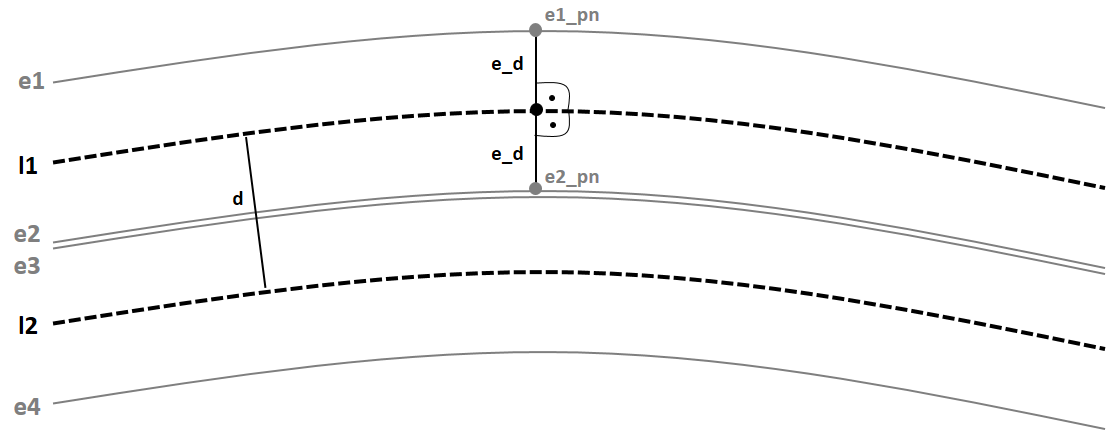
\includegraphics[width=0.75\linewidth]{resources/img/umsetzung/U2/concept_lane_envelope}
    \caption[Konzept Bestimmung Spürhüllen]
            {Konzept Bestimmung Spürhüllen - Ermittlung von Spurbreiten anhand Abstandes paralleler Spuren}
    \label{fig:real2_envelope_definition_concept}
\end{figure}

Die oben beschriebene Definition einer Bahn-Geometrie wird im Spurerkennungs-Modul über eine Klasse
\textit{LaneGeometry} repräsentiert. Diese ist in Abbildung \ref{fig:real2_laneGeometry_ClassDia} dargestellt.
Das Feld \textit{variance} entspricht dem Abstand $e_d$ zwischen der \textit{centerline} und den Hülllinien.

\begin{figure}[H]
    \centering
    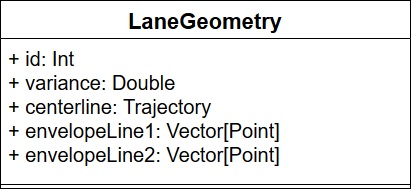
\includegraphics[width=0.38\linewidth]{resources/img/umsetzung/U2/LaneGeometry_ClassDia}
    \caption{Aufbau LaneGeometry Klasse}
    \label{fig:real2_laneGeometry_ClassDia}
\end{figure}

Einen ähnlichen Ansatz zur Bestimmung von Spurbegrenzungslinien verwenden auch Hsieh et al. in ihrer Arbeit.
Sie gehen jedoch, da die von ihnen verwendeten
Aufnahmen von einer statischen Kamera über einer Autobahn stammen, davon aus, dass alle Fahrspuren parallel
zueinander verlaufen. Da das in dieser Arbeit entwickelte Spurerkennungs-Modul mit unterschiedlichen
Aufnahmen und Straßentopologien umgehen können muss, kann diese Annahme nicht getroffen werden.
Nachfolgend werden die Schritte vorgestellt, welche angewandt werden, um in einer Menge von Spuren
jene zu finden, welche parallel zueinander verlaufen. Auf deren Basis werden anschließend die Spurbreiten bestimmt und
die Hülllinien definiert.

\subsubsection{Identifikation paralleler Fahrspuren}
\label{sec:real2_identify_parallel_lanes}

Um in einer Menge von Fahrspuren, welche über Mittellinien repräsentiert werden, jene zu finden, die
parallel zueinander verlaufen, werden in einem ersten Schritt benachbarte Spur-Paare gesucht.
Zwei Fahrspuren $l1$ und $l2$ gelten als benachbart, wenn sich der Start oder das Ende
von Spur $l2$ in einem Bereich mit Radius $\sigma$ um den Start von $l1$ befindet.
Der Wert für $\sigma$ wurde auf Basis der in Deutschland geltenden
\textit{``Richtlinien für die Anlage von Autobahnen''} (\acrshort*{raa}) \cite[]{RAA2008}
und der \textit{``Richtlinien für die Anlage von Landstraßen''} (\acrshort*{ral}) \cite[]{RAL2012} bestimmt.
Diese Regelwerke spezifizieren die in der Bundesrepublik derzeit zulässigen Straßenquerschnitte.
Die in ihnen festgelegten Spurbreiten variieren zwischen 2.75 und 3.75 Metern.
Um auch besonders breite benachbarte Spur-Paare identifizieren zu können, wurde für $\sigma$ der Wert 4m gewählt.

Die auf diese Weise gefundenen Trajektorie-Paare starten oder enden als benachbarte Spuren.
Der Algorithmus welcher prüft, ob zwei Spuren tatsächlich parallel zueinander verlaufen, ist in Listing
\ref{lst:pseudo_checkParallel} beschrieben. Die zu vergleichenden Mittellinien werden jeweils in eine
Reihe von Richtungsvektoren umgewandelt. Anschließend werden paarweise die Winkel zwischen zwei Vektoren
berechnet und die Ergebnisse gemittelt.
Liegt die sich so ergebende Abweichung unter einem Grenzwert $\delta$, so handelt es sich um parallele Spuren.
Zusätzlich wird geprüft, ob die Spuren eine ähnliche Länge besitzen.
\begin{lstlisting}[caption=Pseudocode Überprüfung der Parallelität zweier Mittellinien, language=Pseudo, label=lst:pseudo_checkParallel]
algorithm lanesAreParallel:
  input:  lane-centerline: l1, lane-centerline: l2, delta
  output: True or False

  inOppositeDirections := check (*if*) l1 and l2 run (*in*) opposite directions
  if inOppositeDirections then
    reverse points of centerline l2
  end

  l1DirectionVec := calculate direction vectors (*for*) l1
  l2DirectionVec := calculate direction vectors (*for*) l2
  dirDifferences := calculate pairwise the angle between two direction vectors

  meanDiff := calculate mean angle of deviation between l1 and l2
  lengthDiff := calculate difference between length of l1 and l2

  return meanDiff < delta && lengthDiff >= 0.8
\end{lstlisting}

Für $\delta$ wurde experimentell der Wert 0.1 bestimmt. In den verschiedenen Test-Datensätzen konnten
so zuverlässig parallele Spur-Paare identifiziert werden. Anhand dieser werden im nächsten Schritt
die Spurhüllen bestimmt.

\subsubsection{Berechnung der Hüllen}
\label{sec:real2_create_envelopes}

Bevor für eine Mittellinie die sie umgebende Spurhülle bestimmt werden kann, muss die Breite der Spur
ermittelt werden. Diese ergibt sich, für die im vorherigen Schritt ermittelten parallelen Spur-Paare, aus
deren mittleren Abstand zueinander. Verlaufen zu einer Spurlinie zwei Bahnen parallel, werden
die Abstände zu beiden berechnet und der kleinere Wert wird als Spurbreite gewählt.
Allen Bahnen, welche keine parallele Nachbarspur besitzen, wird das Minimum der im vorherigen Schritt
bestimmten Spurbreiten zugeordnet.
Falls sich in einer Aufnahme keine parallelen Spuren befinden, wird für die Spurbreite ein Standartwert
von 3.5 Metern verwendet, welcher sich ebenfalls aus den RAA und RAL Richtlinien ableitet.

Nachdem Breiten für alle Fahrspuren bestimmt wurden, können die Hülllinien berechnet werden.
Hierzu werden für jeden Punkt der Mittellinie zwei zugehörige Hüllpunkte berechnet.
Das verwendete Vorgehen ist in Abbildung \ref{fig:real2_envelope_point_calculation_concept} dargestellt.

\begin{figure}[H]
    \centering
    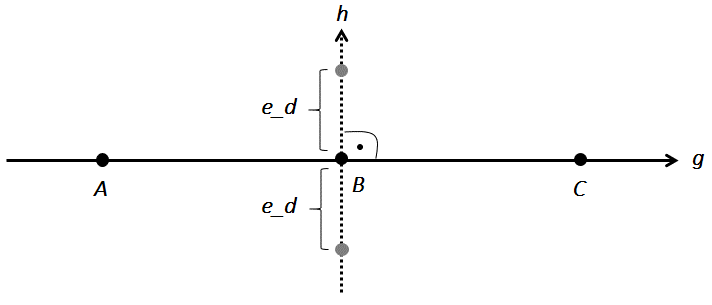
\includegraphics[width=0.5\linewidth]{resources/img/umsetzung/U2/calc_env_point}
    \caption{Konzept Berechnung Spur-Hüllpunkte}
    \label{fig:real2_envelope_point_calculation_concept}
\end{figure}

Um die Hüllpunkte für einen Punkt $B$ einer Mittellinie zu bestimmen, wird eine Gerade $g$ durch die
Punkte $A$ und $C$ gelegt, welche sich vor und hinter $B$ befinden.

\begin{ceqn}
\begin{align}
    g: \vec{x} = \overrightarrow{OA} + t \cdot \overrightarrow{AC}
\end{align}
\end{ceqn}

Anschließend wird durch $B$ eine Gerade $h$ gelegt, welche orthogonal zu $g$ verläuft.

\begin{ceqn}
\begin{align}
    h: \vec{x} = \overrightarrow{OB} + t \cdot \hat{X}
\end{align}
\end{ceqn}

Für ihren Richtungsvektor $\hat{X}$, welcher sich aus $\overrightarrow{AC}$ ergibt, gilt
$\overrightarrow{AC} \cdot \hat{X} = 0$. Da $\hat{X}$ ein Einheitsvektor
ist, können die Hüllpunkte, welche auf $h$ liegen und den Abstand $e_d$ von $B$ besitzten, einfach
bestimmt werden, indem $e_d$ beziehungsweise $-e_d$ für $t$ in die Geradengleichung von $h$ eingesetzt wird.

Auf diese Weise werden die Hülllinien für alle Fahrspuren bestimmt. In Abbildung \ref{fig:real2_results_geometry_definition} sind die
Ergebnisse der Spur-Geometrie-Bestimmung dargestellt. Teil a) zeigt die Spurmittellinien mit ihren
sie umgebenden Hüllen in einem Plot. Teil b) zeigt die in die Anwendung \textit{Vehicle-Tracker} visualisierten Spuren.

\begin{figure}[H]
    \centering
    \subfloat[]{{
        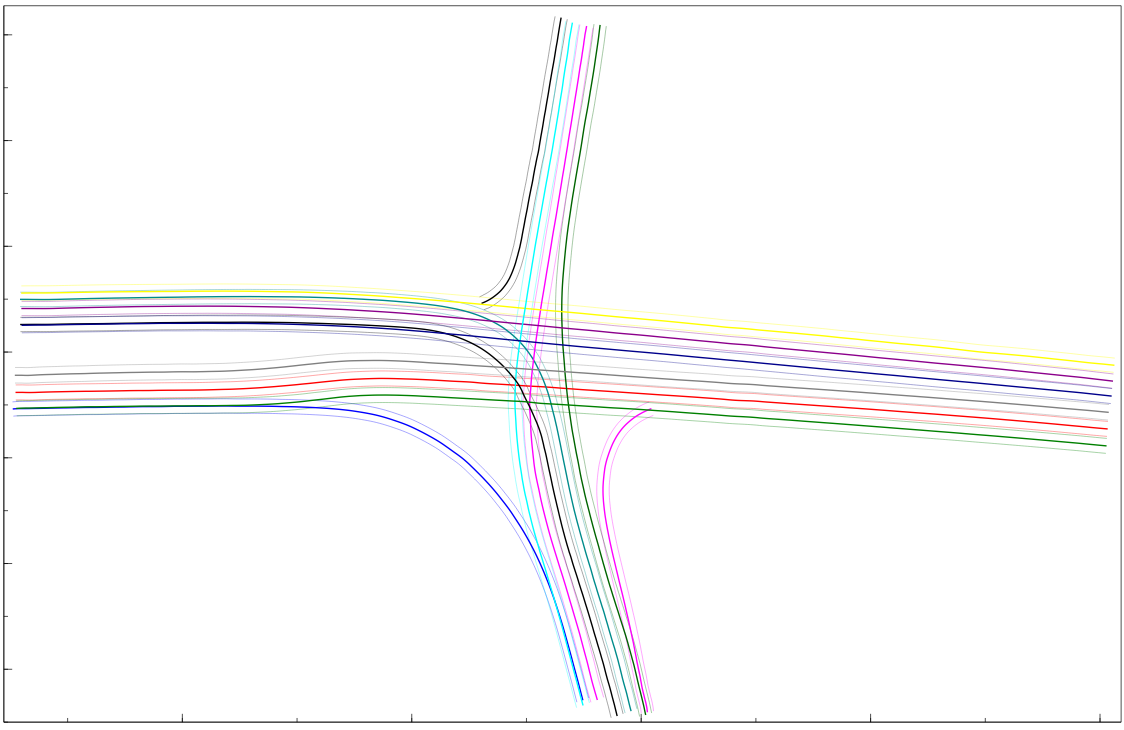
\includegraphics[align=c, width=0.45\linewidth]{resources/img/umsetzung/U2/laneEstimates}
    }}
    \subfloat[]{{
        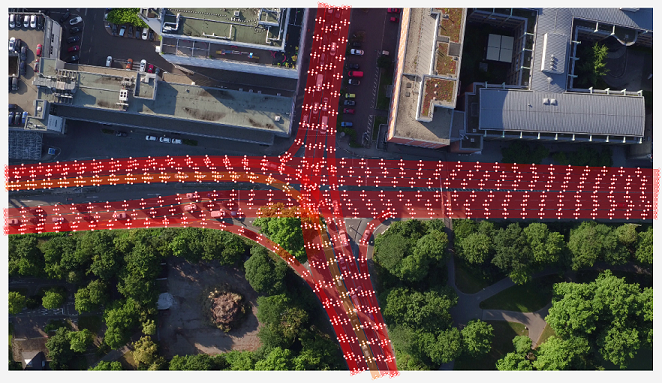
\includegraphics[align=c, width=0.5\linewidth]{resources/img/umsetzung/U2/result_laneEst_Screenshot}
    }}
    \caption[Ergebnisse Spur-Geometrie-Bestimmung]
            {Plot Spur-Geometrien a), Ergebnis Visualisierung Spur-Geometrien in \textit{Vehicle-Tracker} Applikation b)}
    \label{fig:real2_results_geometry_definition}
\end{figure}

Die obige Abbildung zeigt, dass die berechneten Spur-Geometrien in den meisten Fällen bereits gut
mit den realen Spur-Dimensionen übereinstimmen. Bevor die Spuren partitioniert werden, um Überlagerungen
von Fahrspuren zu entfernen, werden in einem weiteren Schritt ``unechte'' Spur-Geometrien entfernt.

\subsubsection{Entfernung von Pseudo-Spur-Geometrien}

Mit Pseudo-Spur-Geometrien sind jene Geometrien gemeint, welche keine real existierende Fahrspur beschreiben.
Am häufigsten treten Pseudo-Fahrspuren in Form von zu kurzen Geometrien auf, oder in Form von Geometrien,
welche einen Spurwechsel beschreiben. Diese zwei Arten von Spur-Geometrien werden daher identifiziert
und entfernt. Beispiele für solche Geometrien sind in Abbildung \ref{fig:real2_unreal_geometries} dargestellt.

\begin{figure}[H]
    \centering
    \subfloat[zu kurze Geometrie (blau)]{{
        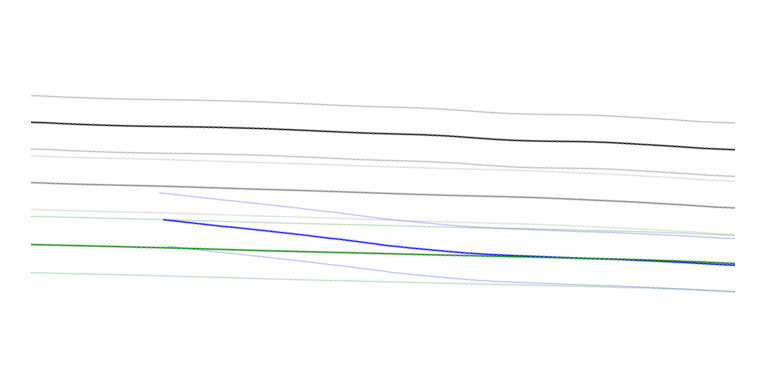
\includegraphics[align=c, width=0.37\linewidth]{resources/img/umsetzung/U2/TooShortLanes}
    }}
    \qquad \qquad
    \subfloat[Spurwechsel Geometrie (rot)]{{
        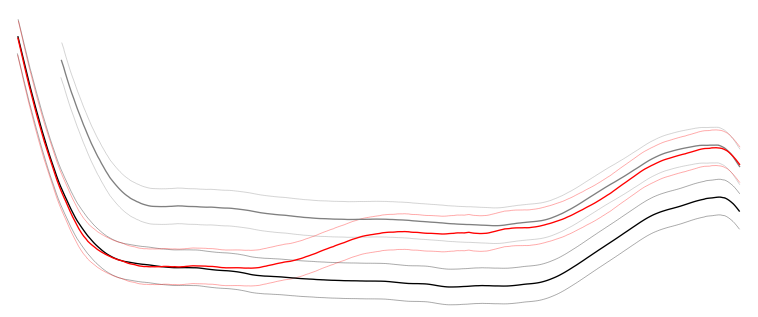
\includegraphics[align=c, width=0.37\linewidth]{resources/img/umsetzung/U2/LaneChangeLanes}
    }}
    \caption{Beispiele Pseudo-Spur-Geometrien}
    \label{fig:real2_unreal_geometries}
\end{figure}

Zu kurz ist eine Spur-Geometrie dann, wenn sie einen Streckenabschnitt beschreibt, welcher
gleichzeitig noch von einer anderen, längeren Spur beschrieben wird. Sie wird daher
gänzlich oder fast gänzlich überlagert. Diese Art von Pseudo-Spuren ist leicht zu identifizieren.
Es wird für jede Spur geprüft, ob eine andere Spur existiert, welche sie zu 95\% oder mehr überlagert.
Wie die Überlagerung von zwei Spuren identifiziert wird, ist in Abschnitt \ref{sec:real2_lane_partitioning}
beschrieben.

Geometrien, welche nicht eine Spur sondern den Wechsel zwischen zwei Spuren darstellen, können
existieren, wenn die Trajektoriedaten viele Spurwechselvorgänge enthalten und in der Cluster-Analyse für
diese ein extra Cluster erstellt wird. Um diese Spuren zu identifizieren, müssen Kriterien eines
Spurwechsel-Vorgangs definiert werden. Diese zeichnen sich primär dadurch aus, dass sie auf einer Spur
$A$ beginnen und auf einer Spur $B$ enden, wobei die Spuren $A$ und $B$ parallel zueinander verlaufen.
Es kann zudem davon ausgegangen werden, dass sich weniger Fahrzeuge auf einer Spurwechsel-Spur bewegen,
als auf den zwei eigentlichen Fahrspuren.
Auf Basis dieser Eigenschaften, ergibt sich der nachfolgende Algorithmus.
\begin{lstlisting}[caption=Pseudocode Identifikation Spurwechsel-Spur, language=Pseudo, label=lst:pseudo_isLaneChangeLane]
algorithm isLaneChangeLane:
  input:  lane-geo: l1, sequence of other lane-geos: otherGeos
  output: True or False

  overlaysAtStart := find lanes (*in*) otherGeos that are overlayed by l1 at its start
  overlaysAtEnd := find lanes (*in*) otherGeos that are overlayed by l1 at its (*end*)

  if overlaysAtStart.nonEmpty && overlaysAtEnd.nonEmpty then:
    a := identify more traveled parallel lanes (*in*) overlaysAtStart
    b := identify more traveled parallel lanes (*in*) overlaysAtEnd
    return a.nonEmpty && b.nonEmpty
  else return false
  end
\end{lstlisting}

Eine Spurwechsel-Spur muss also im Bereich ihres Starts und ihres Endes jeweils mindestens eine andere
mehr befahrene, parallele Fahrspur überlagern.
Nachdem auf diese Weise die Pseudo-Spur-Geometrien entfernt wurden, werden die übrigen partitioniert.

\subsection{Partitionierung von Fahrspuren}
\label{sec:real2_lane_partitioning}

Fahrspuren, welche mithilfe dieser Arbeit erkannt werden, kommen bei der Verkehrsanalyse zum Einsatz.
Unter anderem können mit ihrer Hilfe Spurwechsel- oder Überholvorgänge von Fahrzeugen untersucht werden.
Damit eine solche Analyse sinnvoll ist, dürfen sich Fahrspuren nicht über einen größeren Bereich hinweg überlagern.
Aus diesem Grund werden Spuren, welche in Teilen identisch mit anderen verlaufen, partitioniert. Die
identischen Teile werden verworfen und nur die separaten beibehalten.
Unproblematisch ist es, wenn sich Spuren lediglich kreuzen, ihre Überlagerung also geringfügig ist.
In diesem Fall werden die Spuren nicht partitioniert. Es wird daher zwischen sich überlagernden und sich
kreuzenden Spuren unterschieden. Nachfolgend wird das Verfahren zur Identifikation von sich überlagernden
Fahrspuren und der Partitionierungs-Vorgang beschrieben.

Um Fahrspuren zuverlässig und sinnvoll partitionieren zu können, müssen grundlegend zwei Probleme bewältigt
werden. Es müssen zuerst die sich überlagernden Spur-Paare und deren Schnittpunkte gefunden werden und
anschließend muss für jedes Paar entschieden werden, welche Spur partitioniert wird und welche erhalten bleibt.
Hierzu werden die Spur-Geometrien zuerst in drei Kategorien unterteilt:

\begin{itemize}
    \item isolierte Fahrspuren
    \item primäre Fahrspuren
    \item sekundäre Fahrspuren
\end{itemize}

Isolierte Fahrspuren sind hierbei jene, welche keine Überschneidung mit anderen Spuren besitzen. Primäre
Fahrspuren besitzen keine Überschneidungen untereinander, können sich aber mit anderen Spuren kreuzen oder
von ihnen überlagert werden. In einer Menge von Spur-Geometrien bildet das größte Subset von parallel
zueinander verlaufenden Spuren die primären Fahrspuren. Sekundäre Fahrspuren sind all jene, welche
weder isoliert noch primär sind. In Abbildung \ref{fig:real2_prim_and_sec_lanes} sind die primären und
sekundären Spur-Geometrien der Neckartor-Kreuzung dargestellt.

\begin{figure}[H]
    \centering
    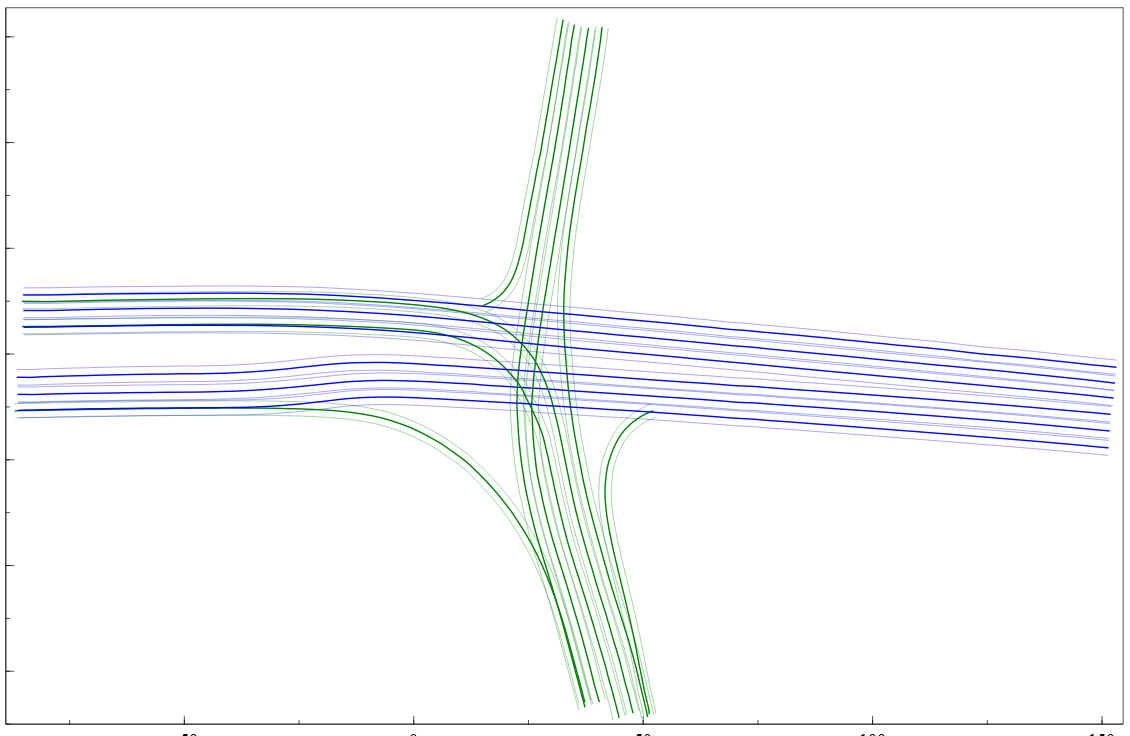
\includegraphics[width=0.4\linewidth]{resources/img/umsetzung/U2/prims_and_secs}
    \caption[Primäre und Sekundäre Spur-Geometrien einer Kreuzung]{Primäre (blau) und sekundäre (grün) Spuren auf einer Kreuzung}
    \label{fig:real2_prim_and_sec_lanes}
\end{figure}

Nachdem die Fahrspuren, anhand der oberen Definition, in die drei Kategorien unterteilt wurden, werden
anschließend die primären und sekundären Spuren nach sich überlagernden Paaren durchsucht.
Zwei Spuren überschneiden sich, wenn, wie in
Abbildung \ref{fig:real2_lane_crossing} zu sehen, die Mittellinie einer Spur innerhalb der Hülle einer
anderen Spur liegt. Die Punkte $b_1$ und $b_2$ entsprechen hierbei den äußeren und inneren Grenzpunkten
der Überschneidung der Mittellinie von $l_2$ mit der Hülle von $l_1$. Zur Bestimmung der Schnittmenge
wird die JTS Topology Suite eingesetzt.

\begin{figure}[H]
    \centering
    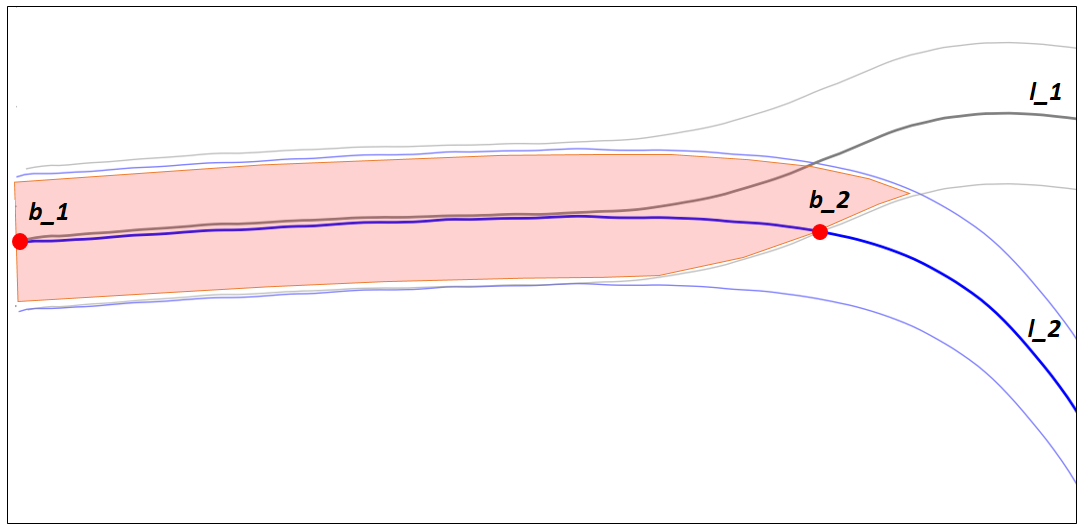
\includegraphics[width=0.5\linewidth]{resources/img/umsetzung/U2/lane_crossing}
    \caption[Überlagerung zweier Spur-Abschnitte]
            {Überlagerung zweier Spur-Abschnitte (roter Bereich) zwischen den Punkten $b_1$ und $b_2$}
    \label{fig:real2_lane_crossing}
\end{figure}

Zwei Spuren $l_1$ und $l_2$ kreuzen sich nicht nur, sondern überlagern sich, wenn der Abschnitt zwischen
den Grenzpunkten $b_1$ und $b_2$ mindestens 10\% der Spurlänge ausmacht. Auf diese Weise werden die
sich überlagernden Spur-Paare und die zugehörigen Schnittpunkte bestimmt.
Aus jeder Überschneidung ergeben sich zwei Spur-Paare.
Im Fall von Abbildung \ref{fig:real2_lane_crossing} wird einerseits $l_1$ von $l_2$ überlagert und andererseits
$l_2$ von $l_1$.

Es kann vorkommen, dass in einem Bereich, in welchem sich zwei Spuren überlagern,
die Mittellinie der einen Spur sich kurzzeitig außerhalb der Hülle der anderen befindet. Bei der Bestimmung
der überlagerten Bereiche, wie oben beschrieben, würde dies dazu führen, dass zwei Überlagerungen statt einer
erkannt werden. Um mit einer solchen Situation korrekt umzugehen, werden die identifizierten Schnittmengen
zwischen zwei Spuren fusioniert, falls die Distanz zwischen ihnen sehr gering ist.
Hierrüber wird sichergestellt, dass eine Spur anschließend nicht fälschlicherweise zweimal
oder zu früh beziehungsweise zu spät partitioniert wird.

Nachdem die sich überlagernden Spur-Paare bestimmt wurden, wird anschließend
entschieden, welche Spur der Paare partitioniert wird und welche erhalten bleibt. Zuerst wird hierzu
überprüft, ob es sich bei einer der Geometrien um eine primäre Fahrspur handelt. Ist dies der Fall, so
bleibt diese erhalten. Existiert in einem Paar keine primäre Spur, so werden verschieden Eigenschaften
der Fahrspuren untersucht, um eine Entscheidung zu treffen, welche Geometrie zu partitionieren ist.
Der hierzu verwendete Algorithmus ist vereinfacht in Listing \ref{lst:pseudo_selectMoreCurvy} dargestellt.

Grundlegen wird zuerst das Krümmungsverhalten der zwei Fahrspuren im Bereich ihres Schnittpunktes untersucht.
Liegt die Differenz der Krümmungen der beiden Spuren oberhalb eines Grenzwertes $\delta$, so wird
jene Spur partitioniert, welche die höhere Krümmung besitzt. Die Annahme ist, dass es sich bei dieser
Spur mit höherer Wahrscheinlichkeit um eine Abbiegespur et cetera handelt, welche in eine gerade Spur übergeht.
Ist die Differenz der Krümmungen kleiner als $\delta$, so verlaufen die zwei Spuren im Bereich des Schnittpunktes
annähernd parallel. In diesem Fall wird entweder anhand der Länge oder der Fahrzeuganzahl entschieden,
welche Spur geteilt wird. Der Anwender der Tracking-Application kann das Verhalten des Algorithmus an dieser Stelle
über einen Parameter steuern. Standardmäßig wird die Anzahl der Fahrzeuge, welche sich auf einer Spur befinden,
als Kriterium verwendet.
\begin{lstlisting}[caption=Pseudocode Auswahl zu partitionierende Fahrspur, language=Pseudo, label=lst:pseudo_selectMoreCurvy]
algorithm selectLaneGeometryForPartitioning:
  input:  lane-geo: l1, lane-geo: l2, boundPoints: bounds
  output: l1 or l2 based on curviness around bounds

  innerBoundPoint := select inner bound point based on distance
                     from b1 and b2 to the edges of l1

  l1Subset := get subset of l1 around innerBoundPoint
  l2Subset := get subset of l2 around innerBoundPoint

  l1CurvMea := estimate curvature of l1Subset
  l2CurvMea := estimate curvature of l2Subset

  if | l1CurvMea - l2CurvMea | > delta then
    partition lane with bigger curvMea
  else
    if check length? then partition shorter lane
    if check vehicle-count? then partition lane with less vehicles
  end
\end{lstlisting}

Im Fall der sich überlagernden Spur-Paare in Abbildung \ref{fig:real2_lane_crossing} ist $b_2$ der \textit{innerBoundPoint}.
Zur Bestimmung der Krümmung einer Fahrspur in einem Bereich, siehe Listing \ref{lst:pseudo_selectMoreCurvy}
Zeile 11 + 12, wird der Winkel $\varphi$ zwischen den Richtungsvektoren des Anfang und Endes der Teilspur berechnet.
Er ergibt sich anhand Gleichung \ref{eq_angle_skalar}.

\begin{ceqn}
\begin{align}
\label{eq_angle_skalar}
    \varphi=\arccos \frac{\vec a \cdot \vec b}{|\vec a| |\vec b|}
\end{align}
\end{ceqn}

Nachdem alle zu teilenden Spuren und die zugehörigen Grenzpunkte
bestimmt wurden, folgt die eigentliche Partitionierung. Aus den Spur-Geometrien werden alle Bereiche
entfernt, welche zwischen den zwei Grenzpunkten einer Überlagerung liegen. In Abbildung \ref{fig:real2_lane_crossing}
wird so beispielsweise der rot gekennzeichnete Bereich der Spur $l_2$ zwischen $b_1$ und $b_2$ entfernt.

Abbildung \ref{fig:real2_results_partitioning} zeigt das Ergebnis der Spur-Partitionierung im Fall des
\textit{Neckartor} Datensatzes. Es wurden alle Spur-Überlagerungen entfernt.

\begin{figure}[H]
    \centering
    \subfloat[]{{
        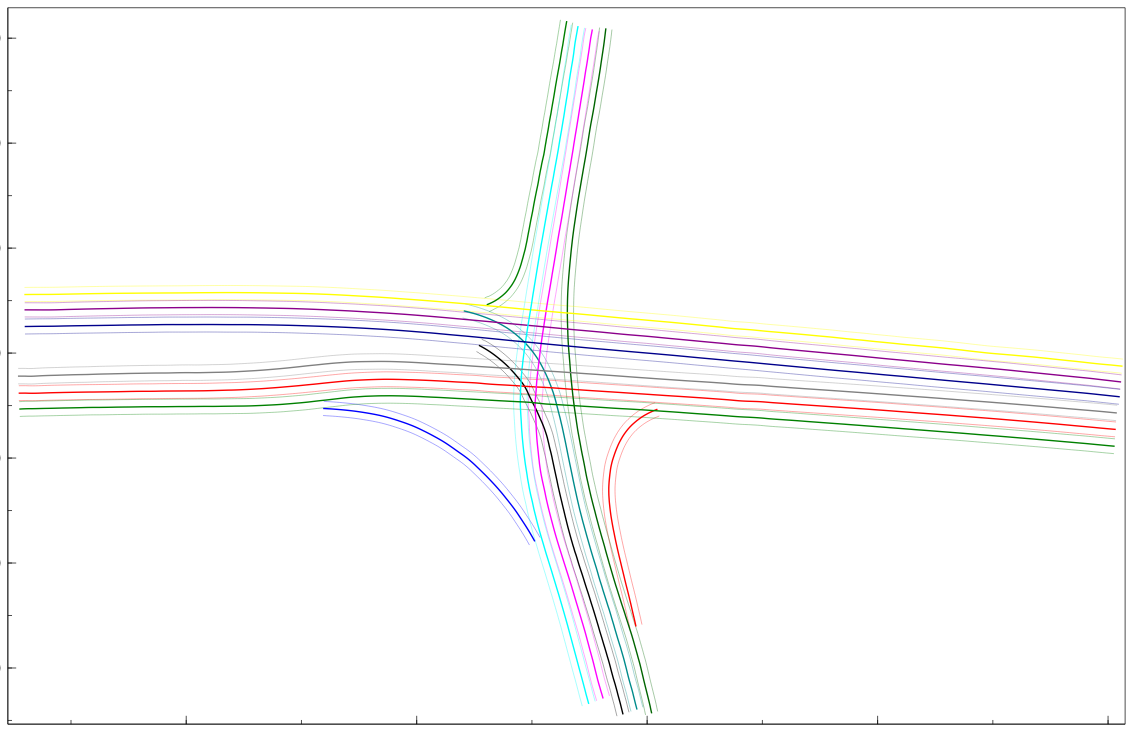
\includegraphics[align=c, width=0.4\linewidth]{resources/img/umsetzung/U2/partitionedLanes}
    }}
    \qquad
    \subfloat[]{{
        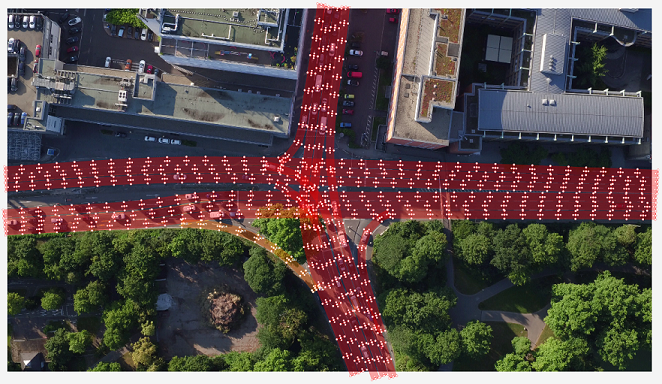
\includegraphics[align=c, width=0.45\linewidth]{resources/img/umsetzung/U2/result_lanePartitioned_Screenshot}
    }}
    \caption[Ergebnisse Spur-Partitionierung]
            {Plot partitionierte Spur-Geometrien a), Visualisierung Ergebnis in der Anwendung \textit{Vehicle-Tracker} b)}
    \label{fig:real2_results_partitioning}
\end{figure}

Die so ermittelten Spur-Geometrien entsprechen in den meisten Fällen bereits dem gewünschten Ergebnis,
da sie die realen Fahrspur-Verläufe gut wiederspiegeln und keine Überlagerungen mehr existieren.
In einigen Szenarien kann es jedoch vorkommen, dass nach der Geometrie-Ermittlung und der Partitionierung
die Fahrspur-Geometrien die reale Straßentopologie noch nicht korrekt abbilden. Aus diesem Grund werden die
Spur-Geometrien in einem weiteren Schritt nochmals optimiert.

\subsection{Optimierung der Spur-Geometrien}
\label{sec:real2_lane_geo_opt}

Die nach dem Partitionierungs-Schritt vorliegenden Spur-Geometrien besitzen in einigen Fällen noch Defekte.
Das am häufigsten auftretende Problem ist, dass die Spur-Geometrien nicht breit genug sind.
Abbildung \ref{fig:real2_pre_opt} zeigt beispielsweise die Spur-Geometrien eines Straßen-Abschnitts,
in welchem sich rechts zwei parallele Fahrspuren befinden, welche sich links in vier Spuren aufteilen.
Es ist erkennbar, dass die zwei Fahrspuren zu Beginn nicht direkt aneinander angrenzen
und daher in diesem Abschnitt nicht breit genug sind. In diesem Fall resultiert die zu niedrige Fahrbahnbreite
aus der starken Überlagerung der vier Spur-Geometrien im rechten Bereich vor deren Partitionierung.
Diese verursacht eine falsche Schätzung der Spur-Breite (siehe Abschnitt \ref{sec:real2_define_lane_envelope}).

\begin{figure}[H]
    \centering
    \fbox{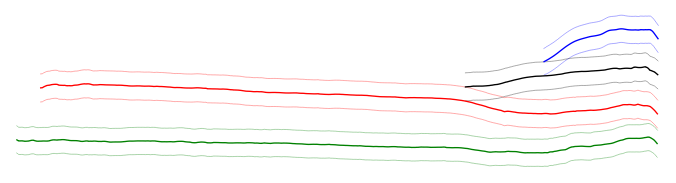
\includegraphics[align=c, width=0.7\linewidth]{resources/img/umsetzung/U2/laneOpt_partitioned_pre}}
    \caption[Beispiel zu schmale Spur-Geometrien]
            {Beispiel zu schmale Spur-Geometrien - Parallele rote und schwarze Spur-Geometrien grenzen nicht aneinander an}
    \label{fig:real2_pre_opt}
\end{figure}

Um Effekte wie diesen zu korrigieren, werden nach der Partitionierung nun nochmals die Breiten aller Spur-Geometrien
neu bestimmt. Im Gegensatz zu dem verwendeten Vorgehen aus Abschnitt \ref{sec:real2_define_lane_envelope},
bei welchem für jede Spur eine feste Breite berechnet wurde, wird diese nun für jeden Punkt der Spur einzeln
berechnet. Hierdurch wird es möglich, dass beispielsweise die rote und grüne Spur aus Abbildung \ref{fig:real2_pre_opt}
zu Beginn breiter sind, als an ihrem Ende.

Der zur Bestimmung der neuen Spurbreiten eingesetzte Algorithmus hat vereinfacht den nachfolgenden Ablauf:

\begin{itemize}
    \item Wähle eine Spur-Geometrie $l$
    \item Für jeden Punkt $p$ der Mittellinie von $l$ mit Position $i$:
    \begin{itemize}
        \item Suche korrespondierende Punkte $P_k = \{pk_0\ ...\ pk_n\}$ auf benachbarten Spuren
        \item Wähle einen benachbarten Punkt $pk_j \in P_k$
        \item Verwende die Distanz zwischen $p$ und $pk_j$ als Spurbreite von $l$ an Position $i$
    \end{itemize}
\end{itemize}

Entscheidend bei diesem Verfahren ist es, den richtigen Punkt $pk_j$ auszuwählen. Dieser muss grundsätzlich
auf jener Spur liegen, welche im Bereich des Punktes $p$ parallel zu $l$ verläuft und ihr am nächsten liegt.

Nachdem auf diese Weise für eine Spur punktweise die neuen Breiten bestimmt wurden, werden diese noch mithilfe
eines gleitenden Mittelwert Verfahrens geglättet. Anschließend werden neue Spurhüllen, mittels dem in
Abschnitt \ref{sec:real2_create_envelopes} vorgestellten Vorgehen, erzeugt.
Das Ergebnis der Geometrie-Optimierung für den Fall der in Abbildung \ref{fig:real2_post_opt} enthaltenen Spuren,
ist nachfolgend dargestellt.

\begin{figure}[H]
    \centering
    \fbox{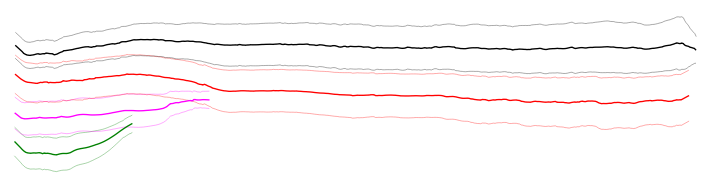
\includegraphics[align=c, width=0.7\linewidth]{resources/img/umsetzung/U2/laneOpt_optimized}}
    \caption[Ergebnis Spur-Optimierung]
            {Ergebnis Spur-Optimierung - rote und schwarze Spuren grenzen aneinander an}
    \label{fig:real2_post_opt}
\end{figure}

Die Fahrspurerkennung ist nach dem Optimierungsschritt abgeschlossen. Auf Basis der vorliegenden
Spur-Geometrien können anschließend die Fahrspuren in die Anwendung \textit{Vehicle-Tracker} eingefügt werden.

\subsection{Anlegen der Fahrspuren in der Anwendung Vehicle-Tracker}

Nachdem die Spur-Geometrien auf Basis der Fahrzeugtrajektorien bestimmt wurden, müssen diese in einem
finalen Schritt noch in das von der \textit{Vehicle-Tracker} Applikation verwendete Datenmodell zur Repräsentation von
Fahrspuren überführt werden. Dieses Vorgehen ist nachfolgend beschrieben.

Wie bereits zu Beginn der Arbeit erwähnt, wurden Fahrspuren bislang manuell über die Benutzeroberfläche
der \textit{Vehicle-Tracker} Anwendung angelegt. Das verwendete Datenmodell, welches auch weiterhin
für die automatisch erkannten Spuren verwendet wird, ist in Abbildung \ref{fig:real2_lane_datamodell} dargestellt.

\begin{figure}[H]
    \centering
    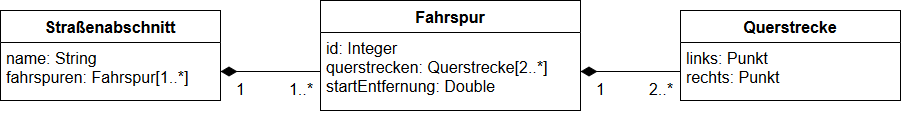
\includegraphics[align=c, width=0.85\linewidth]{resources/img/umsetzung/U2/Fahrspurmodell}
    \caption{Datenmodell der Spurdefinition}
    \label{fig:real2_lane_datamodell}
\end{figure}

Eine Fahrspur in einem Streckenabschnitt besteht aus mindestens zwei \textit{Querstrecken}. Jede Querstrecke
legt über zwei Punkte die Breite der Fahrspur auf einer bestimmten Höhe der Spur fest. Eine Fahrspur
kann aus beliebig vielen Querstrecken bestehen, wodurch es möglich ist, die Fahrspuren beliebig detailliert
zu definieren.

Die Fahrspuren und Querstrecken werden im Fall der automatisch erkannten Fahrbahnen anhand der Spur-Hüllen
definiert. Über Punkt-Paaren der beiden Hülllinien (siehe Abbildung \ref{fig:real2_laneGeometry_ClassDia}),
werden Querstrecken erstellt.
Da eine Fahrspur möglichst über die kleinste Menge an Querstrecken beschrieben werden soll, welche die
Geometrie der Bahn zuverlässig abbildet, wird nicht für jedes Hüllpunkt-Paar eine Querstrecke definiert.
Die Anzahl und Distanz zwischen den Querstrecken richtet sich nach der Krümmung der Spuren. Zur Beschreibung
einer geraden Fahrspur werden weniger Querlinien benötigt, als zur Beschreibung einer Kurve.
Zur Bestimmung der Querstrecken werden daher die Hülllinien abschnittsweise untersucht und jeweils
die Richtungsänderungen zwischen aufeinanderfolgenden Abschnitten betrachtet. Hierzu wird erneut
die Gleichung \ref{eq_angle_skalar} eingesetzt.
Überschreitet die Richtungsänderung einer Hülle einen Grenzwert von $\phi = 0.02$, so wird eine neue
Querstrecke erstellt. Anderenfalls verläuft die Spur im untersuchten Bereich annähernd gerade.
In Abbildung \ref{fig:real2_lanes_trackerApplication} ist das Ergebnis der Spurerstellung dargestellt.
Es ist gut zu erkennen, dass im Fall der geraden Fahrspuren der Autobahn nur wenige Querstrecken zur
Definition der Spur verwendet werden, und für die gekrümmten Spuren deutlich mehr.

\begin{figure}[H]
    \centering
    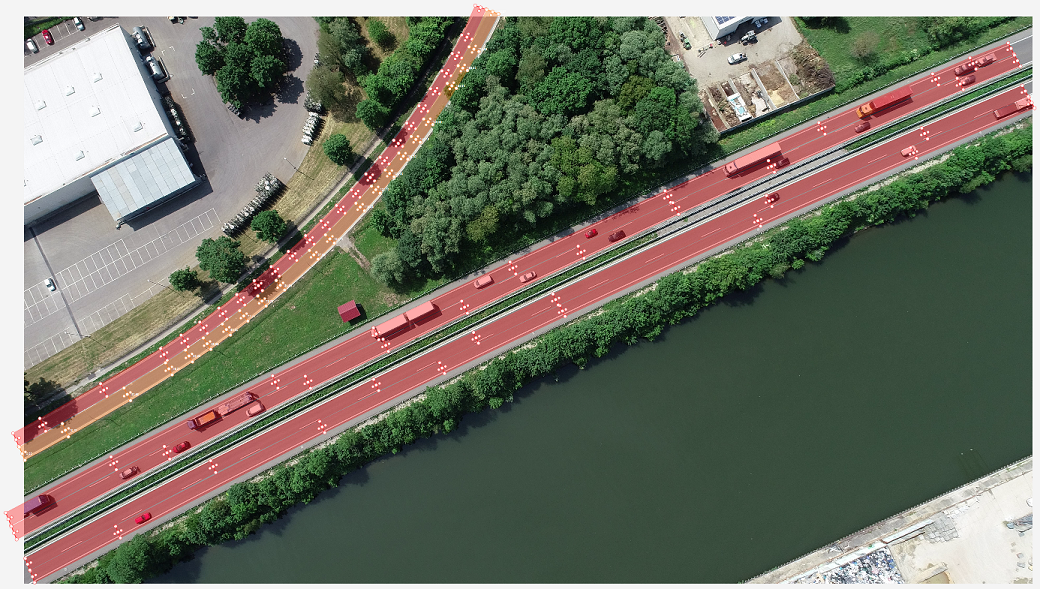
\includegraphics[align=c, width=0.6\linewidth]{resources/img/umsetzung/U2/LaneCreator_Example}
    \caption{Angelegte Fahrspuren in der \textit{Vehicle-Tracker} Anwendung}
    \label{fig:real2_lanes_trackerApplication}
\end{figure}

Ein Vorteil, welcher sich durch die Weiterverwendung des in Abbildung \ref{fig:real2_lane_datamodell}
dargestellten Datenmodells ergibt, ist, dass Benutzer weiterhin Spuren manuell anlegen können und automatisch
detektierte Fahrbahnen sich nachträglich noch leicht modifizieren lassen. Falls eine vom Algorithmus erkannte
Spur also beispielsweise in einem Abschnitt zu schmal oder zu breit ist, kann dies leicht vom Nutzer korrigiert
werden.

Nachdem die Fahrspuren in der \textit{Vehicle-Tracker} Anwendung angelegt wurden, können sie zur Auswertung
des Verkehrs in der Luftbeobachtung verwendet werden.
Die Ergebnisse und Qualität des in diesem Kapitel vorgestellten Algorithmus, werden im nachfolgenden
Auswertungskapitel vorgestellt.